\chapter{Business Processes}
In this chapter we analyze a set of business processes which are
fundamental activities inside our organization, we provide an analysis of
these processes and the results of a simulation.

Before going in deeper details in analyzing the processes is useful to get
a wider view on the organization structure.
AllSpark, is an enterprise with the aim to develop and deploy services in
the IT area.

Our services can vary from a common web hosting service to very complex and
possibly innovative security systems, and therefore we need to distinguish
the different departments in which our organization is divided.

\section{Departments and structure}
Our organization is divided in several activity areas, each one of them
contains the processes and the people needed to operate in a specific
field.

In the AllSpark organization is possible to identify the following
different areas:
\begin{description}
\item[Administration:] This part of the enterprise manages the
administrative part of the organization, takes marketing decision, follows
the public relations with external partners, solves bureaucratic issues
and is responsible for the financial operations.
\item[Project Management:] This segment of the organization is involved in
the core processes of manage the different phases of project development.
These activities represent a set of core functions in the organizations
aims, is this sector, in facts, which is responsible for the actual
implementation of our products.
\item[Working resource management:] The processes and resources which are
involved in this sector provide support for the maintenance of hardware
and software. There are processes dedicated to reparation as to the update
of different resources.
\item[Course and Certification:] AllSpark, as an enterprise, organizes
courses for developers and sysadmins. For this reason a particular division
of the organization is dedicated to the management of courses and seminars.
\item[Research and Development:] The employees in this area work actively in
the research's world, mainly in security related field. In our organization
this section is vital for improving our products and develop new one.
\end{description}

The company map in figure \ref{2img:cmap} depicts clearly the business processes
performed in each section and how them are related to each other.

\begin{figure}
\begin{centering}
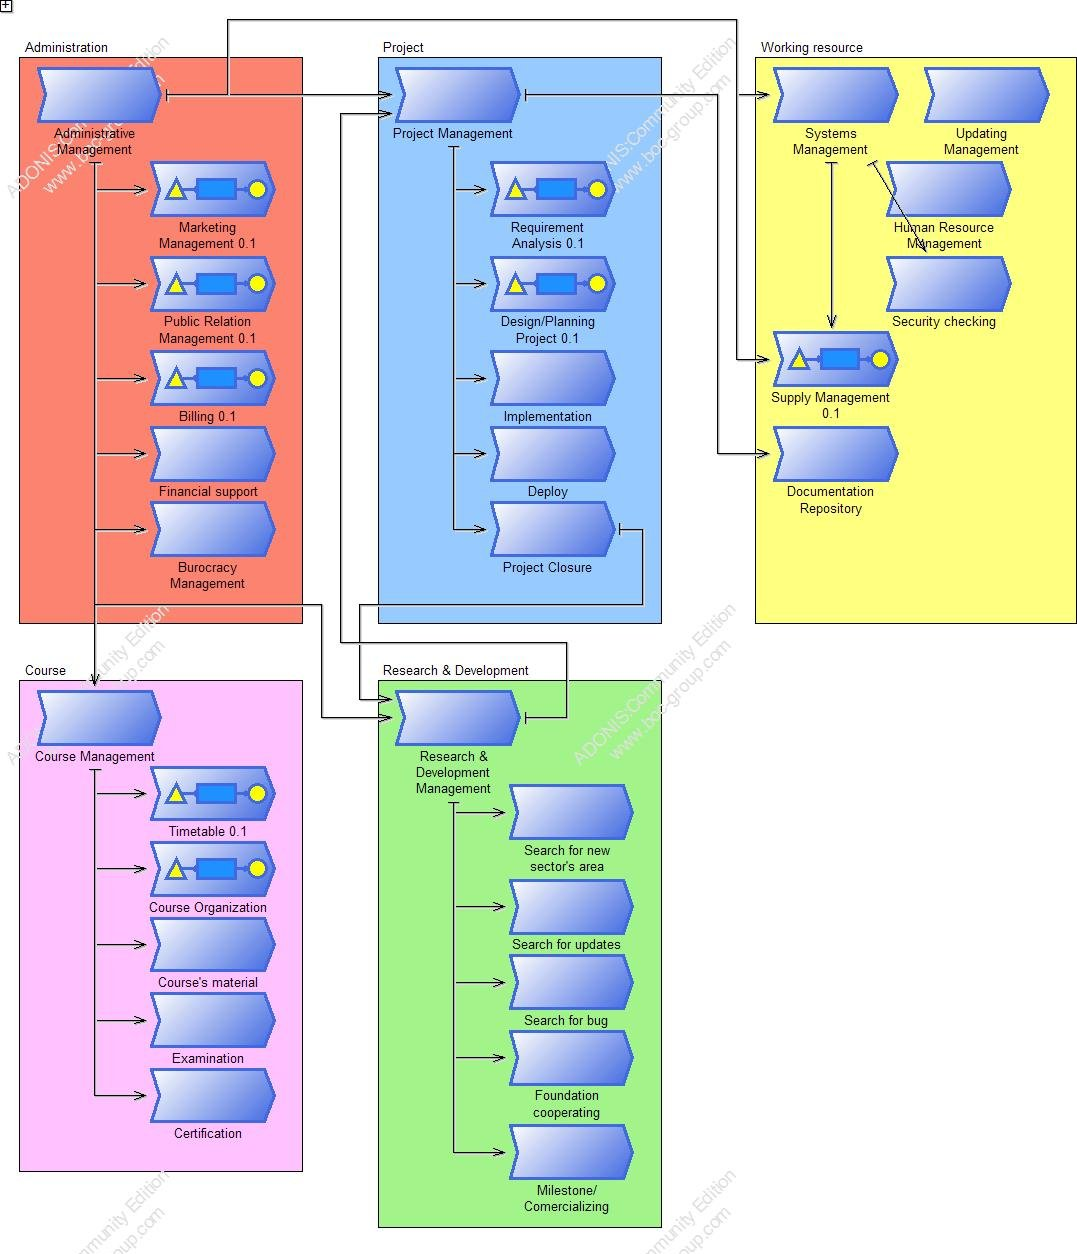
\includegraphics[scale=0.40]{assign2/adonis/imgs/companymap.jpg}
\caption{AllSpark company map}
\label{2img:cmap}
\end{centering}
\end{figure}

\paragraph{Billing}
This process provides support for the definition of the appropriate
remuneration for the service supplied.
This process takes into account the history of project development and the
details defined in the contract, in order to check if they match or if some
extra features have been during the development phase.

Image \ref{2img:billing} shows how this process is realized in practice,
focusing on the resources used and the targets for each activity.
The goal of this process is to provide a fair billing to the customer,
balanced on the services actually delivered.

\begin{figure}[ht!]
\begin{centering}
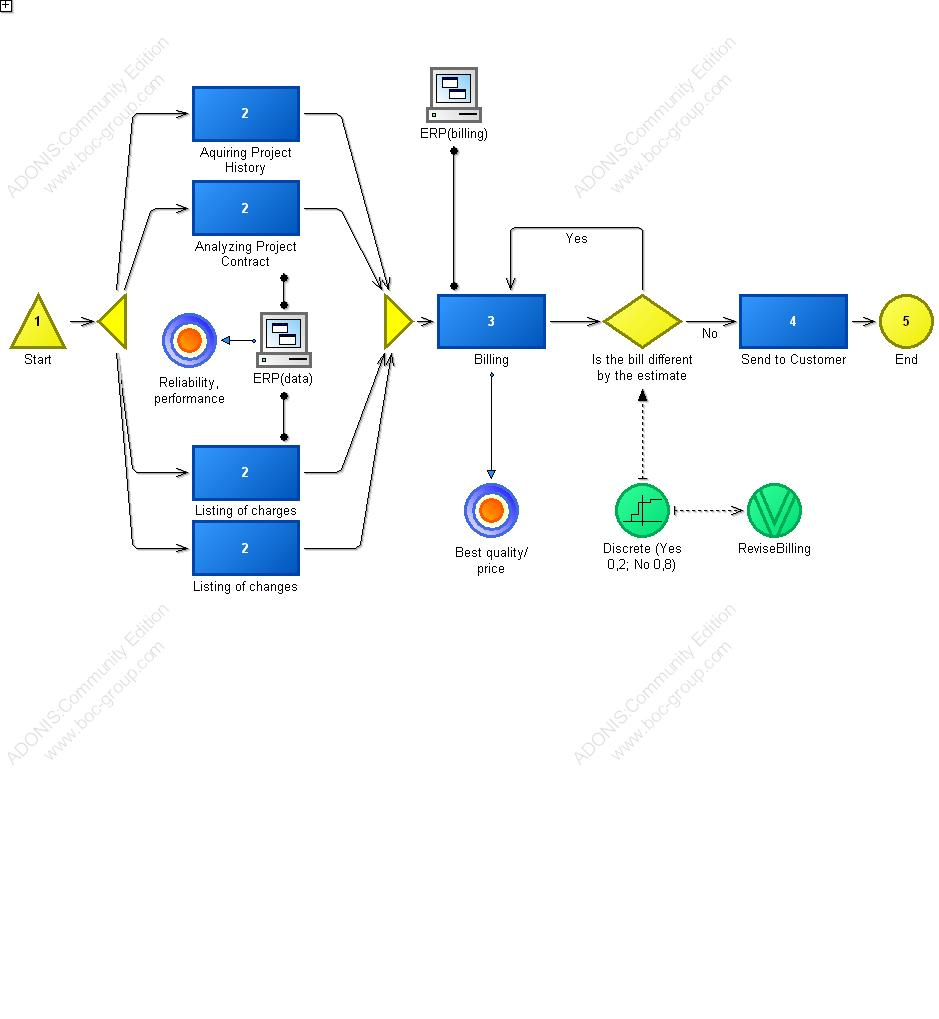
\includegraphics[scale=0.50]{assign2/adonis/imgs/billing.jpg}
\caption{AllSparks billing process}
\label{2img:billing}
\end{centering}
\end{figure}

